\begin{center}
    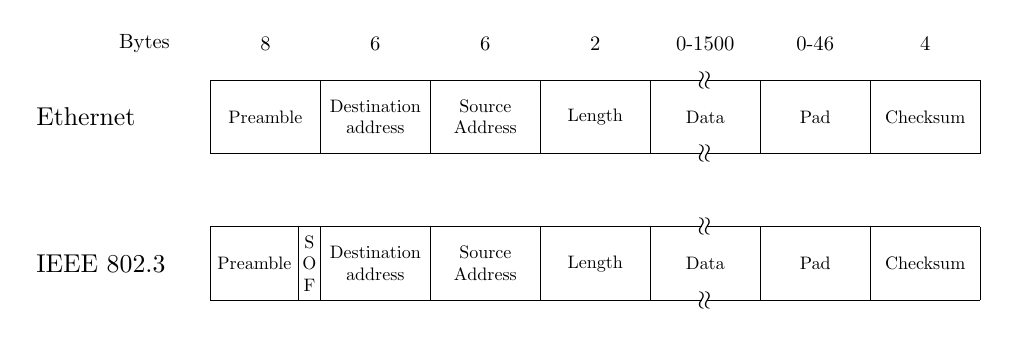
\begin{tikzpicture}[scale=0.931,every node/.style={scale=0.931}]
        %%%%%%% Blocchi 1 %%%%%%%%
        \draw (0,0) -- ++(6.7,0) ++ (.08,0) -- (10.5,0);
        \draw (0,1) -- ++(6.7,0) ++ (.08,0) -- (10.5,1);
        \node[rotate=90] at (6.75,0) {$\approx$};
        \node[rotate=90] at (6.75,1) {$\approx$};
        \draw (1.2,0) -- ++(0,1);

        \foreach \x in {0,1.5,...,10.5}
            \draw (\x,0) -- ++(0,1);

        %%%%%%% Blocchi 2 %%%%%%%%
        \draw (0,2) -- ++(6.7,0) ++ (.08,0) -- (10.5,2);
        \draw (0,3) -- ++(6.7,0) ++ (.08,0) -- (10.5,3);
        \node[rotate=90] at (6.75,2) {$\approx$};
        \node[rotate=90] at (6.75,3) {$\approx$};

        \foreach \x in {0,1.5,...,10.5}
            \draw (\x,2) -- ++(0,1);

        %%%%%%% Tipo frame %%%%%%%
        \node[anchor=west] at (-2.5,2.5) {Ethernet};
        \node[anchor=west] at (-2.5,0.5) {IEEE 802.3};

        %%%%%%%% Testo 1 %%%%%%%%%
        \node[scale=0.7] at (.6,.5) {Preamble};
        \node[scale=0.7,text width=0.27cm,align=center] at (1.35,.5) {S O F};
        \node[scale=0.7,text width=2cm,align=center] at (2.25,.5) {Destination address};
        \node[scale=0.7,text width=2cm,align=center] at (3.75,.5) {Source Address};
        \node[scale=0.7,text width=2cm,align=center] at (5.25,.5) {Length};
        \node[scale=0.7,text width=2cm,align=center] at (6.75,.5) {Data};
        \node[scale=0.7,text width=2cm,align=center] at (8.25,.5) {Pad};
        \node[scale=0.7,text width=2cm,align=center] at (9.75,.5) {Checksum};

        %%%%%%%% Testo 2 %%%%%%%%%
        \node[scale=0.7] at (.75,2.5) {Preamble};
        \node[scale=0.7,text width=2cm,align=center] at (2.25,2.5) {Destination address};
        \node[scale=0.7,text width=2cm,align=center] at (3.75,2.5) {Source Address};
        \node[scale=0.7,text width=2cm,align=center] at (5.25,2.5) {Length};
        \node[scale=0.7,text width=2cm,align=center] at (6.75,2.5) {Data};
        \node[scale=0.7,text width=2cm,align=center] at (8.25,2.5) {Pad};
        \node[scale=0.7,text width=2cm,align=center] at (9.75,2.5) {Checksum};

        %%%%%%%%% Bytes %%%%%%%%%%
        \node[scale=0.8] at (-0.9,3.5) {Bytes};
        \node[scale=0.8] at (0.75,3.5) {8};
        \node[scale=0.8] at (2.25,3.5) {6};
        \node[scale=0.8] at (3.75,3.5) {6};
        \node[scale=0.8] at (5.25,3.5) {2};
        \node[scale=0.8] at (6.75,3.5) {0-1500};
        \node[scale=0.8] at (8.25,3.5) {0-46};
        \node[scale=0.8] at (9.75,3.5) {4};
    \end{tikzpicture}
\end{center}